\documentclass[
 reprint,
 amsmath,amssymb,
 aps,
]{revtex4-1}

\usepackage{graphicx}
\usepackage{dcolumn}
\usepackage{bm}

\begin{document}

\preprint{APS/123-QED}

\title{Ising 2D}

\author{Felipe Gonzalez}

\affiliation{%
 Departamento de F\'\i sica, Facultad de Ciencias Exactas y Naturales, Universidad de Buenos Aires,\\
 Pabell\'on I, Ciudad Universitaria, 1428 Buenos Aires, Argentina.
}

\date{\today}

\begin{abstract}
Se estudio la evoluci\'on de un sistema de Ising de dos dimensiones para
distintos tama\~nos de red y temperaturas. Se buscaron los exponentes cr\'iticos
de la transici\'on de fase que sufre la magnetizaci\'on media de la muestra en
funci\'on de la temperatura, llegando a los valores esperados por la teor\'ia,
siendo estos,

$$
\left \{
  \begin{matrix}
    \gamma = (1.70 \pm 0.10) \\
    \beta = (0.108 \pm 0.002) \\
    \alpha = (-0.002 \pm 0.002)
  \end{matrix}
\right.
$$

\end{abstract}

\pacs{45.70.Vn, 89.65.Lm}

\maketitle

\section{Introducci\'on}

El modelo de Ising es un modelo f\'isico desarrollado para estudiar el
comportamiento de materiales ferromagnéticos, pero que es de inter\'es para el
estudio de fen\'omenos cr\'iticos en general. Es el modelo paradigm\'atico para
el estudio de transiciones de fase, presentando una de ellas cuando la
temperatura del sistema decrece a un valor cr\'itico tal que surge
magnetizaci\'on espont\'anea.

Este modelo fue inventado por el f\'isico Wilhelm Lenz, que lo concibió
como un problema para su alumno Ernst Ising para demostrar que el sistema
presentaba una transici\'on de fase. Ising demostró que en una dimensión
no existía tal transici\'on de fase, resolviéndolo en su tesis de 1924. El modelo
bidimensional de Ising de retícula cuadrada solo pudo ser descripto
analíticamente mucho más tarde, por Lars Onsager, que demostró que
efectivamente se encuentra una transici\'on de fase a un temperatura cr\'itica
$T_c > 0$\cite{Onsager}.

\section{El modelo}

El modelo de Ising se constituye por un arreglo bidimensional de espines
est\'aticos con orientaci\'on \textit{up} o \textit{down}, los cuales
evolucionan de manera "aleatoria" en funci\'on de la temperatura de la muestra
y la energ\'ia de interacci\'on entre espines. Esta evoluci\'on esta
caracterizada por un Metropolis - Hastings, el cual ser\'a explicado en la
proxima secci\'on.

\subsection{Algoritmo de Metropolis Hastings}

El algoritmo de Metropolis Hastings, tambien conocido como Markov-Chain
Monte Carlo (MCMC) es un metodo para obtener secuencias de muestras aleatorias
de una distribuci\'on de probabilidad de la cual sampleo directo es dificil.

Este consiste en tomar muestras de una distribuci\'on de la siguiente manera.
Se propone un nuevo estado, $x'$ el cual tiene una probabilidad $P(x')$, y se
define el siguiente elemento de la cadena como:

$$
x_{i + 1} = \left \{
\begin{matrix}
  x' \; \text{si } \frac{P(x')}{P(x_i)} > 1 \\
  \left \{ \begin{matrix}
    x' \; \text{con probabilidad }\frac{P(x')}{P(x_i)} \\
    x_i \; \text{con probabilidad }1 - \frac{P(x')}{P(x_i)}
\end{matrix}
  \right \}
 \;\;\;\; \text{si } \frac{P(x')}{P(x_i)} < 1
\end{matrix}   \right.
$$

Usando este algoritmo, empezando de alguna muestra $x_0$, y luego de un periodo
de termalizaci\'on, se llega a una tira de muestras cuya distribuci\'on de
probabilidad corresponde con la de sampleo. Se entiende termalizaci\'on como la
cantidad de pasos necesarios para que el sistema "olvide" su estado inicial, y
asi el sampleo sea representativo de la funci\'on de probabilidad que la caracteriza.

\subsection{Modelo de Ising}

El modelo de Ising estudiado consiste en una red bidimensional infinita,
rellena de espines con proyecci\'on \textit{up} o \textit{down}, caracterizada
por el siguiente Hamiltoniano.

\begin{equation}
  H = - \sum_i^N s_i B - J \sum_{<i, j>} s_i s_j,
\end{equation}

siendo, $s_i$ la proyecci\'on de cada esp\'in, $B$ un campo magn\'etico externo,
$J$ la energia de interacci\'on entre cada par de esp\'i y $<i, j>$ simboliza la
sumatoria que cuenta \'unicamente los primeros vecinos de cada esp\'in. Vemos que
no contamos con una energ\'a cin\'etica, por lo que cada esp\'in se encuentra
est\'atico.

Existen soluciones anal\'iticas para este problema. Para el caso de $J = 0, B
\neq 0$ tenemos que el problema se puede resolver plantenado un sistema
can\'onico, en el cual cada esp\'in no interactua por lo que se puede plantear
lo siguiente.

As\'i, tenemos que la funci\'on de partici\'on can\'onica es

\begin{equation}
  Q = \sum \exp^{-\beta H} = \sum_{s_1} \sum_{s_2} ... \sum_{s_N} \exp^{\beta B \sum_{i = 1}^N s_i}
\end{equation}
\begin{equation}
  Q = (\sum_{s_1} \exp^{\beta B  s_1}) ^ N = (\exp^{B\beta} + \exp^{-B\beta}) ^ N,
\end{equation}

y por lo tanto la energ\'ia del sistema es

\begin{equation}
  E = -\frac{\partial}{\partial \beta} \ln Q = -\frac{N}{kT}\tanh{\frac{B}{kT}}.
\end{equation}

Otro caso muy interesante es el caso de $B = 0, J \neq 0$. Para este caso,
Onsager\cite{Onsager} demuestra que existe $T_c = \frac{}{}$ tal que para $T <
T_c$ se tiene que ocurre magnetizaci\'on espontanea, que corresponde a una
transici\'on de fase de segundo orden (continua, con derivada discontinua) cuyo
par\'ametro de orden es la magnetizaci\'on media de la red. Tenemos que esta
soluci\'on dice que la magnetizaci\'on media de la red en function de $J$ es

\begin{equation}
  <s_i> =
  \left \{
    \begin{matrix}
      0 \; \text{si } J^* < J_C \\
      [1 - \sinh^{-4} (2J^*)]^{\frac{1}{8}} \; \text{si } J^* > J_C \\
    \end{matrix}
  \right . ,
\end{equation}

con $J^* = \frac{J}{kT} = J\beta$. Sobre este trabajo se utiliza la siguiente
convenci\'on, en la cual se toma $k_b = 1$, $J \rightarrow \frac{J}{T}$ y $B
\rightarrow \frac{B}{T}$, de manera que $J^* \equiv J$. Tenemos que $J_C$ es tal
que:

\begin{equation}
  2 \tanh(2 J_C) = 1 \Rightarrow J_C \simeq 0.44
\end{equation}

\section{\label{simulations}Simulaciones num\'ericas}

Para realizar simulaciones num\'ericas cuya validez se sostenga, se tuvo
especial cuidado con las siguientes cuestiones.

Se comenz\'o por realizar un estudio sobre longitud de correlaci\'on y
termalizacion de la red en funcion de los distintos valores de temperatura, en
pos de asegurar que las muestras tomadas sean representativas de la temperatura
en la cual se setea el sistema. Para esto se realizo un barrido para $J \in
[0.1, 0.6]$, en una red de lado $L = 32$ con $300.000$ pasos,
con $300.000 >> L^2 = 1024$, con la intenci\'on de estar completamente seguro
de que para cada $J$ se llega a un estado representativo de la temperatura y
que no corresponde a un transitorio, sino al estacionario. Sobre la figura
\ref{termalizacion} se puede ver la magnetizaci\'on media de la muestra en
funci\'on de cada paso, para $J < J_c$ y $J > J_c$. Vemos que para temperaturas
bajas $(J > J_c)$ tenemos que la cantidad de pasos para termalizar el sistema
se vuelve muy grande superando ampliamente el estimado inicial de $L^2$,
mientras que para $J < J_c$ el sistema llega a un estado representativo de la
temperatura en relativamente pocos casos.

\begin{figure}
  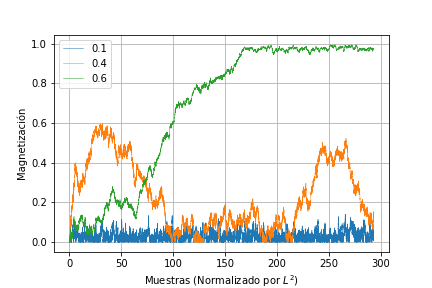
\includegraphics[width=1.0\columnwidth]{images/termalizacion.png}
  \caption{Magnetizacion media de la muestra en funci\'on del numero de pasos,
    normalizado por $L^2$. Vemos que para temperaturas bajas $(J = 0.6)$ el
    n\'umero de pasos necesarios para termalizar es muy alto (del orden de 100
    veces $L^2$) mientras que para temperaturas altas $(J = 0.1)$ el sistema
    termaliza en relativamente pocos pasos. Tenemos el caso de $J = 0.4
    \simeq J_C$ en el cual se puede ver que la muestra esta altamente
    correlacionada y que no llega a un estado realmente estacionario.}
  \label{termalizacion}
\end{figure}

Otro fen\'omeno interesante surge al estudiar la correlaci\'on de las
mediciones. Vemos en la figura \ref{termalizacion} que para $J \simeq J_c$, la
muestra muestra una gran correlaci\'on para varios pasos, ya que se puede ver
una especie de "forma funcional" para puntos separados por muchos mas de $L^2$
pasos, comparado con el caso de $J < J_c$. Comparando las longitudes de
correlaci\'on (figura \ref{correlation}) se vuelve muy claro como para $J_c$
es importante que el sampleo de magnitudes ocurra cada una gran cantidad de
pasos, en pos de asegurar descorrelaci\'on entre mediciones.

\begin{figure}
  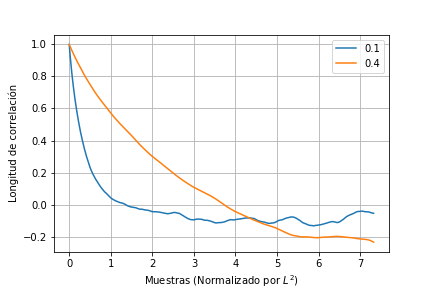
\includegraphics[width=1.0\columnwidth]{images/correlation.png}
  \caption{Longitud de correlation de las muestras de magnetizaci\'on en
    funci\'on del numero de pasos, normalizado por $L^2$. Vemos que para
    temperaturas altas $(J = 0.1)$ el n\'umero de pasos para descorrelacionar
    las mediciones es del orden de $L^2$, mientras que para $J \simeq J_C$ se
    vuelve casi 5 veces mayor.}
  \label{correlation}
\end{figure}

\section{Resultados}

\subsection{Exponentes cr\'iticos}

Comenzamos por analizar la red para $B = 0$ y $J\in[0.1, 0.6]$,
con un paso de $0.01$ y $100.000$ puntos por paso. A todas las mediciones se les
dio $150.000$ pasos para termalizar, y se dejaron $3.000$ entre mediciones en pos
de asegurar la descorrelacion entre mediciones.

\begin{figure}
  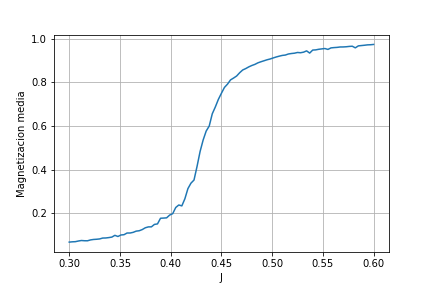
\includegraphics[width=1.0\columnwidth]{images/magnetization_vs_j.png}
  \caption{Magnetizacion media de la muestra en funci\'on de $J$. Vemos como
    para temperaturas bajas ($J > J_C \simeq 0.44$) se pierde la suavidad,
    debido a que la muestra se vuelve muy dificil de termalizar.}
  \label{magnetization_vs_j}
\end{figure}

El valor medio del absoluto de la magnetizaci\'on en funcion de $J$ se puede
encontrar en la figura \ref{magnetization_vs_j} . Vemos que efectivamente se
puede ver que para $J<J_c \simeq 0.44...$ se encuentra que la muestra sufre una
ruptura espontanea de simetr\'ia, y la muestra empieza a tener una
magnetizaci\'on media total distinta de cero aunque no exista campo magn\'etico.
Tenemos que de esta distribuci\'on se puede obtener el exponente cr\'itico
$\beta$, ya que sabemos que

$$\frac{<M>}{N} \propto (1 - \frac{T}{T_C})^\frac{1}{8} \Rightarrow
  \beta_{TEO} = \frac{1}{8}.$$

\begin{figure}
  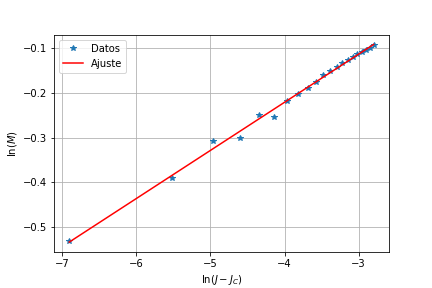
\includegraphics[width=1.0\columnwidth]{images/ajuste_beta.png}
  \caption{Ajuste lineal del logaritmo de la magnetizaci\'on media de la
    muestra en funci\'on de $J - J_c$, con $J_C = 0.44$ el valor te\'orico.
    Tenemos que el ajuste da un valor de $\beta = (0.108 \pm 0.002)$, un poco
    por debajo del valor te\'orico de $\frac{1}{8} = 0.125$.}
  \label{ajuste_beta}
\end{figure}

Sobre la figura \ref{ajuste_beta} se puede ver un ajuste logar\'itmico sobre la
parte de la curva correspondiente, llegamos a que $\beta = (0.108 \pm 0.002)$,
un poco por debajo del valor te\'orico de $\frac{1}{8} = 0.125$.

M\'as interesante de estudiar son las funciones respuesta del sistema, siendo
particularmente interesante en este caso la susceptibilidad magn\'etica $\chi =
\frac{\partial M}{\partial B}|_{B \rightarrow 0} \simeq <M^2> - <M>^2$.

\begin{figure}
  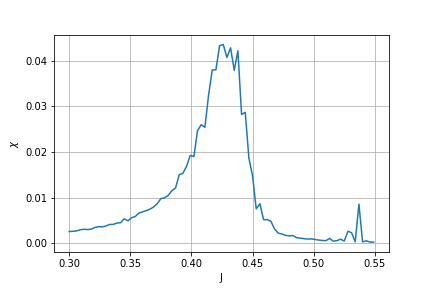
\includegraphics[width=1.0\columnwidth]{images/chi_vs_j.png}
  \caption{Susceptibilidad magn\'etica en funcion de $J$. Vemos como tenemos un
  pico as\'imetrico en $J \simeq 0.44$, correspondiente a la transici\'on de
  fase.}
  \label{chi_vs_j}
\end{figure}

En la figura \ref{chi_vs_j} tenemos la susceptibilidad magn\'etica en funci\'on
de $J$. Vemos como tenemos un pico en la zona de $J \simeq J_C$, cuyo valor si
la red fuera infinita diverge. Sabemos que la susceptibilidad magn\'etica sigue
una ley de potencias, siendo esta cerca del punto cr\'itico proporcional a $|T -
T_c|^{-\gamma}$, con el valor te\'orico de $\gamma$ siendo $\gamma_{TEO} =
\frac{7}{4}$.

\begin{figure}
  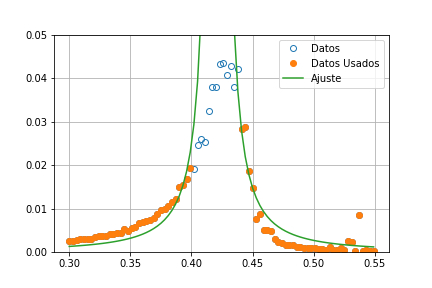
\includegraphics[width=1.0\columnwidth]{images/ajuste_gamma.png}
  \caption{Ajuste no lineal de la susceptibilidad magn\'etica en funcion de $J$.
  Tenemos que el ajuste corresponde a $\gamma = (1.70 \pm 0.10)$, valor
  indistinguible del valor te\'orico $\gamma_{TEO} = \frac{7}{4}$ y $J_C =
  (0.421 \pm 0.001)$, menor al te\'orico, a causa de los efectos de red finita.}
  \label{ajuste_gamma}
\end{figure}

En la figura \ref{ajuste_gamma} tenemos un ajuste lineal sobre la curva de la
susceptibilidad magn\'etica en funci\'on de $J$, llegando a un valor de $\gamma
= (1.70 \pm 0.10)$ y $J_C = (0.421 \pm 0.001)$. Vemos que el $\gamma$ encontrado es indistinguible del valor te\'orico. Adem\'as, tenemos que el $J_C$ es mas
chico que el te\'orico, lo que es esperado debido a los efectos de red finita.

\begin{figure}
  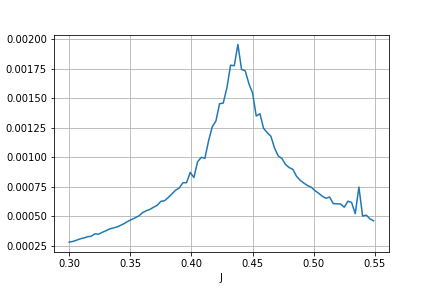
\includegraphics[width=1.0\columnwidth]{images/c_vs_j.png}
  \caption{Capacidad calor\'ifica de la red en funci\'on de $J$.}
  \label{c_vs_j}
\end{figure}

\begin{figure}
  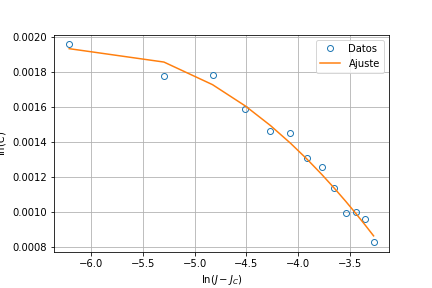
\includegraphics[width=1.0\columnwidth]{images/ajuste_alpha.png}
  \caption{Ajuste sobre el logaritmo de la capacidad cal\'orifica, en funci\'on
    del logaritmo de la diferencia entre $J$ y $J_C$. El ajuste se realiza
    permitiendo una dependencia cuadr\'atica, se encuentra entonces que $\alpha
    = (-0.002 \pm 0.002)$, compatible con $0$ como lo indica la teor\'ia.}
  \label{ajuste_alpha}
\end{figure}

La soluci\'on exacta de Onsager nos indica que $C \propto \ln (1 -
\frac{T}{T_C})$, lo que implica que no existe ley de potencia para $C$. Podemos
ver la capacidad calor\'ifica de la red en funci\'on de $J$ en la figura
\ref{c_vs_j}. Si uno quiere forzar la existencia de una ley de pontencias y
realiza un ajuste, encuentra efectivamente que $\alpha = (-0.002 \pm 0.002)$,
como se puede ver en la figura \ref{ajuste_alpha}.

De esta manera, tengo que se cumple que:

$$
\left \{
  \begin{matrix}
    \gamma = (1.70 \pm 0.10) \\
    \beta = (0.108 \pm 0.002) \\
    \alpha = (-0.002 \pm 0.002)
  \end{matrix}
\right. ,
$$
por lo que puedo conseguir el exponente $\nu$ usando la relaci\'on universal $\nu d = 2 - \alpha$, llegando a que $\nu = 1$.

% Esquema:
% Parte estandar
  % 1. Magnetizacion en funcion de J para L = 32
% Funciones respuesta
  % 1. Chi en funcion de J para L = 32
  % 2. C en funcion de J para L = 32
% Exponentes
  % Beta = 1/8, M = (1 - T / T_c) ^ beta
  % nu sale de relacion universal, nu.d = 2 - a (a = 0) ==> nu = 1
  % gamma = 7/4, sale de , chi = |T - T_C|^-gamma
  % Busco medir Z, coeficiente critico dinamico, gamma / nu.
  % Ademas se cumple que a + 2 beta + gamma = 2.
% Caso Antiferro
% Frustracion
% Dependencia con L
  % Grafico de magentizacion media en funcion de J para distintos L (se "suaviza")
  % Grafico de chi en funcion de J para distintos L (se corre para la izquierda)

\subsection{Efectos de red finita}

Existen consecuencias por simular un sistema infinito como uno finito pero
peri\'odico. Estas consecuencias se conocen como efecto de red finita, y en
este caso son predominantemente 2.

Uno de los efectos de red finita es la suavizaci\'on de las curvas de
magnetizacion en funci\'on de $J$. En la figura \ref{magnetization_vs_l} se
puede ver este fen\'omeno.

\begin{figure}
  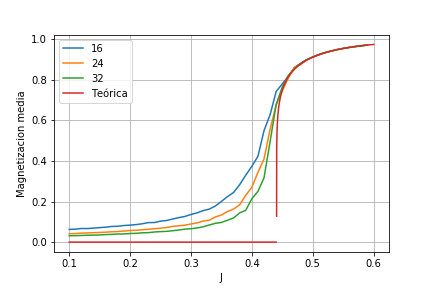
\includegraphics[width=1.0\columnwidth]{images/magnetization_vs_l.png}
  \caption{Magnetizaci\'on media de la red en funci\'on de $J$ para distintos
  valores de $L$, adem\'as de la curva te\'orica. Se puede ver claramente como
  la finitud de la red incide sobre la suavidad sobre la transici\'on.}
  \label{magnetization_vs_l}
\end{figure}

Otro efecto de red finita que se puede ver es la disminucion de $J_C$ en
funci\'on de $L$, se tiene que para $L$ finito se "adelanta" la transici\'on.
Esto se hace especialmente claro en el gr\'afico de la susceptibilidad
magn\'etica, como se puede ver en la figura \ref{chi_vs_l}. Se puede ver como
las curvas son trasladadas hacia la derecha a medida que crece $L$.

\begin{figure}
  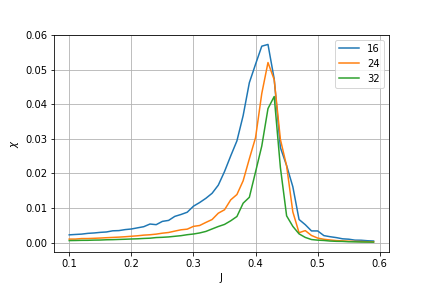
\includegraphics[width=1.0\columnwidth]{images/chi_vs_l.png}
  \caption{Susceptibilidad magn\'etica de la red en funci\'on de $J$ para distintos valores de $L$. Se puede ver claramente como la finitud de la red incide sobre las curvas, desplazandolas hacia menores $J$.}
  \label{chi_vs_l}
\end{figure}

\section{\label{conclusions}Conclusiones}

Se realizo un estudio sobre una red bidimensional cuadrada de Ising, en el rango
de $\frac{J}{kT} \in [0.1, 0.6]$, para lados de $L \in {4, 16, 24, 32, 64}$. Se
observo la transicion de fase de primer orden sobre la magnetizacion de la
muestra, siendo el par\'ametro de orden la temperatura de la muestra, cuyos
exponentes cr\'iticos medidos fueron

$$
\left \{
  \begin{matrix}
    \gamma = (1.70 \pm 0.10) \\
    \beta = (0.108 \pm 0.002) \\
    \alpha = (-0.002 \pm 0.002)
  \end{matrix}
\right. ,
$$

todos indistinguibles con los predichos te\'oricamente excepto por $\beta$, el cual difiere en un 10\%.

Se estudiaron tambien los efectos de red finita, pudiendo identificar como la
finitud de la red tiene como principales efectos suavizar y adelantar las
transiciones.

\appendix
\bibliography{apspaper}

\end{document}
